\documentclass[a4paper, 12pt]{article}
\input{../preamble.tex}

% Диаграммы Эйлера--Венна: #1 --- команды заливки, #2 --- подпись
\newcommand{\venn}[2]{%
\begin{tikzpicture}[scale=0.55]
  \begin{scope}
    #1
  \end{scope}
  \draw (0,0) circle (1) (1.2,0) circle (1);
  \node at (-0.45,0) {$A$};
  \node at (1.65,0) {$B$};
  \node at (0.6,-1.5) {#2};
\end{tikzpicture}}
\newcommand{\dokstart}{$\triangle$\ }
\newcommand{\dokend}{\ $\blacktriangle$}
\usepackage{tikz}
\usetikzlibrary{decorations.pathreplacing}
\setlength{\tabcolsep}{4pt}
% Без колонтитулов и номеров страниц (было \newpagestyle из titlesec — конфликтовал с fancyhdr)
\pagestyle{empty}

\begin{document}
\begin{center}
{\large КОНСПЕКТ ЛЕКЦИЙ}

ПО ДИСЦИПЛИНЕ <<МАТЕМАТИЧЕСКИЙ АНАЛИЗ>>
\end{center}

\tableofcontents
\label{contents}

\pagebreak

\section{Элементы теории множеств и логики}

\subsection{Множества}

\emph{Множество} --- произвольная совокупность определённых предметов нашей
интуиции или интеллекта, которые можно отличить один от другого и которые
представляются как единое целое.
\hfill --- Георг Кантор

Под \underline{множеством} понимают любую определённую совокупность объектов,
различимых между собой. Объекты, из которых составлено множество, ---
\underline{элементы множества}.

$A, B, X$ --- множества; \quad $a, b, x, y$ --- элементы множества.
\[
  \boxed{x \in X, \quad y \notin X}
\]

Когда строится теория множеств, используется интуитивный принцип объёмности
или аксиома экстенсиональности.

Два множества равны тогда и только тогда, когда они состоят из одних и тех же
элементов: каждый элемент первого множества является элементом второго,
а каждый элемент второго --- элементом первого.

Множество называется \textbf{конечным}, если оно состоит из конечного числа
элементов.

Множество называется \textbf{бесконечным}, если оно содержит бесконечное число
элементов.

Если множество не содержит ни одного элемента, то оно называется
\textbf{пустым} ($\varnothing$).

В конкретных задачах элементы всех множеств берутся из некоторого одного
достаточно широкого множества $U$, которое называется
\underline{универсальным} \underline{множеством} (универсумом).

\subsubsection{Способы задания множества}

\begin{enumerate}[noitemsep]
  \item перечислением элементов;
  \item рекурсивно (перечисляющей процедурой);
  \item характеристическим свойством.
\end{enumerate}

\textbf{Пример 1 (рекурсивно).}
\begin{enumerate}[noitemsep]
  \item $3 \in X$;
  \item если $x \in X$, то $\dfrac{1}{x} \in X$ и $(1 - x) \in X$;
  \item других элементов в этом множестве нет.
\end{enumerate}
\[
  X = \left\{ 3;\ \tfrac{1}{3};\ -2;\ -\tfrac{1}{2};\ \tfrac{2}{3};\ \tfrac{3}{2} \right\}
\]

\textbf{Пример 2 (характеристическим свойством).} % в оригинале подписан как «Пример 3»
\[
  A = \{\, x : x \in \mathbb{Z},\ x^{2} \le 4 \,\} = \{-2;\ -1;\ 0;\ 1;\ 2\}
\]
\[
  B = \{\, x : x \in \mathbb{N},\ x \,\vdots\, 2 \,\} = \{2;\ 4;\ 6;\ \dots\}
\]

Чтобы избежать парадоксов, задание множеств ограничивают специальной
аксиоматикой. В частности, используют \underline{аксиому регулярности}:
\[
  X \in X \ \text{--- недопустимо!} \qquad \fbox{Парадокс брадобрея!!!}
\]

\subsubsection{Операции над множествами}

\textbf{Соглашения:}
\begin{itemize}[noitemsep]
  \item $\Longleftrightarrow$ --- <<тогда и только тогда>>;
  \item $\exists x$ (квантор существования) --- существует $x$ такой, что\dots;
  \item $\forall x$ (квантор всеобщности) --- для любого (всякого) $x$;
  \item $\Longrightarrow$ --- следует.
\end{itemize}

Множество $A$ называется \textbf{подмножеством} множества $B$, если
$\forall x \in A\ (x \in B)$. При этом говорят, что $A$ содержится в $B$
или $B$ включает $A$:
\[
  \boxed{A \subseteq B}
\]

Если $A \subseteq B$ и $B \subseteq A$, то множества называются \textbf{равными}
($A = B$).

Множества удобно изображать с помощью кругов Эйлера (диаграмма Венна):
\begin{center}
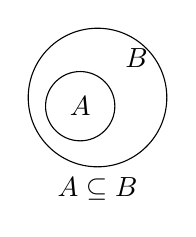
\begin{tikzpicture}[scale=0.55]
  \draw (0,0) circle (1.6);
  \draw (-0.4,-0.2) circle (0.8);
  \node at (-0.4,-0.2) {$A$};
  \node at (0.9,0.9) {$B$};
  \node at (0,-2.1) {$A \subseteq B$};
\end{tikzpicture}
\end{center}

\textbf{Объединение множеств} $A \cup B$:
\[
  A \cup B = \{\, x : x \in A \vee x \in B \,\}
\]
\begin{center}
\venn{\fill[gray!40] (0,0) circle (1) (1.2,0) circle (1);}{$A \cup B$}
\end{center}

\textbf{Пересечение множеств} $A \cap B$ (обозначают также $AB$):
\[
  A \cap B = \{\, x : x \in A \wedge x \in B \,\}
\]
\begin{center}
\venn{\clip (0,0) circle (1); \fill[gray!40] (1.2,0) circle (1);}{$A \cap B$}
\end{center}

\textbf{Разность множеств} $A \setminus B$:
\begin{center}
\venn{\clip (0,0) circle (1); \fill[gray!40, even odd rule] (0,0) circle (1) (1.2,0) circle (1);}{$A \setminus B$}
\qquad
\venn{\clip (1.2,0) circle (1); \fill[gray!40, even odd rule] (0,0) circle (1) (1.2,0) circle (1);}{$B \setminus A$}
\end{center}

\textbf{Симметричная разность множеств}:
\[
  A \,\triangle\, B = (A \setminus B) \cup (B \setminus A)
\]
\begin{center}
\venn{\fill[gray!40, even odd rule] (0,0) circle (1) (1.2,0) circle (1);}{$A \,\triangle\, B$}
\end{center}

\textbf{Дополнение множества} относительно универсального множества:
\[
  \overline{A} = U \setminus A = CA
\]
\begin{center}
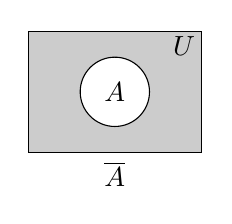
\begin{tikzpicture}[scale=0.55]
  \fill[gray!40] (-2,-1.4) rectangle (2,1.4);
  \fill[white] (0,0) circle (0.8);
  \draw (-2,-1.4) rectangle (2,1.4);
  \draw (0,0) circle (0.8);
  \node at (0,0) {$A$};
  \node at (1.6,1.05) {$U$};
  \node at (0,-1.9) {$\overline{A}$};
\end{tikzpicture}
\end{center}

\subsubsection{Свойства операций}

\begin{itemize}[noitemsep]
  \item \textbf{коммутативность}:
    \[ A \cup B = B \cup A, \qquad A \cap B = B \cap A; \]
  \item \textbf{ассоциативность}:
    \[ (A \cup B) \cup C = A \cup (B \cup C), \qquad
       (A \cap B) \cap C = A \cap (B \cap C); \]
  \item \textbf{дистрибутивность}:
    \[ (A \cup B) \cap C = (A \cap C) \cup (B \cap C), \qquad
       (A \cap B) \cup C = (A \cup C) \cap (B \cup C); \]
  \item \textbf{идемпотентность}:
    \[ A \cup A = A, \qquad A \cap A = A; \]
  \item \textbf{законы де Моргана} (правила двойственности):
    \[ \overline{A \cup B} = \overline{A} \cap \overline{B}, \qquad
       \overline{A \cap B} = \overline{A} \cup \overline{B}; \]
  \item \textbf{поглощение}:
    \[ A \cup (A \cap B) = A, \qquad A \cap (A \cup B) = A; \]
  \item свойства $\overline{A}$, $\varnothing$ и $U$: % заголовок пункта в оригинале зачёркнут
    \[
      \begin{aligned}
        A \cup \overline{A} &= U, & A \cup U &= U, \\
        A \cap \overline{A} &= \varnothing, & A \cap U &= A, \\
        A \cup \varnothing &= A, & U \cup \varnothing &= U, \\
        A \cap \varnothing &= \varnothing, & U \cap \varnothing &= \varnothing.
      \end{aligned}
    \]
\end{itemize}

\subsection{Алгебра высказываний}

\textbf{Высказывание} --- такое предложение, которое либо истинно, либо ложно.
Высказывание не может быть одновременно и истинным, и ложным.

Высказывания обозначают заглавными буквами.

Сопоставив истинному высказыванию символ $1$, а ложному --- $0$, введём
функцию $\lambda$, заданную на совокупности всех высказываний и отвечающую
следующему требованию:
\[
  \lambda(P) =
  \begin{cases}
    1, & \text{если } P \text{ --- истинно};\\
    0, & \text{если } P \text{ --- ложно}.
  \end{cases}
\]
Функцию $\lambda$ называют \textbf{функцией истинности}, а значение
$\lambda(P)$ --- \textbf{логическим значением} высказывания $P$.

\begin{itemize}
  \item \textbf{Отрицанием} высказывания $P$ называется новое высказывание,
    обозначаемое $\neg P$, которое истинно, если высказывание $P$ ложно,
    и ложно, если высказывание $P$ истинно.
    \[ \boxed{\neg P,\quad \overline{P},\quad !P} \]

  \item \textbf{Конъюнкцией} двух высказываний $P$ и $Q$ называется новое
    высказывание, обозначаемое $P \wedge Q$ или $P \,\&\, Q$, которое истинно
    лишь в единственном случае, когда истинны оба высказывания $P$ и $Q$,
    и ложно во всех остальных случаях (логическое~$\times$).
    \begin{center}
    \begin{tabular}{c|c|c}
      $\lambda(P)$ & $\lambda(Q)$ & $\lambda(P \wedge Q)$ \\ \hline
      0 & 0 & 0 \\
      0 & 1 & 0 \\
      1 & 0 & 0 \\
      1 & 1 & 1 \\
    \end{tabular}
    \end{center}

  \item \textbf{Дизъюнкцией} двух высказываний $P$ и $Q$ называется новое
    высказывание, обозначаемое $P \vee Q$, которое истинно тогда и только
    тогда, когда истинно хотя бы одно из высказываний $P$ или $Q$, и ложно
    в единственном случае, когда оба высказывания $P$ и $Q$ ложны
    (логическое~$+$).
    \begin{center}
    \begin{tabular}{c|c|c}
      $\lambda(P)$ & $\lambda(Q)$ & $\lambda(P \vee Q)$ \\ \hline
      0 & 0 & 0 \\
      0 & 1 & 1 \\
      1 & 0 & 1 \\
      1 & 1 & 1 \\
    \end{tabular}
    \end{center}

  \item \textbf{Импликацией} двух высказываний $P$ и $Q$ называется новое
    высказывание, обозначаемое $P \Rightarrow Q$ (<<если $P$, то $Q$>>,
    <<из $P$ следует $Q$>>), которое ложно в единственном случае, когда
    высказывание $P$ истинно, а $Q$ ложно, а во всех остальных случаях ---
    истинно.
    \begin{center}
    \begin{tabular}{c|c|c}
      $\lambda(P)$ & $\lambda(Q)$ & $\lambda(P \Rightarrow Q)$ \\ \hline
      0 & 0 & 1 \\
      0 & 1 & 1 \\
      1 & 0 & 0 \\
      1 & 1 & 1 \\
    \end{tabular}
    \end{center}

  \item \textbf{Эквиваленцией} двух высказываний $P$ и $Q$ называется новое
    высказывание $P \Leftrightarrow Q$ (<<тогда и только тогда>>), которое
    истинно в том и только в том случае, когда оба высказывания $P$ и $Q$
    одновременно истинны или оба ложны, а во всех остальных случаях --- ложно.
    \begin{center}
    \begin{tabular}{c|c|c}
      $\lambda(P)$ & $\lambda(Q)$ & $\lambda(P \Leftrightarrow Q)$ \\ \hline
      0 & 0 & 1 \\
      0 & 1 & 0 \\
      1 & 0 & 0 \\
      1 & 1 & 1 \\
    \end{tabular}
    \end{center}
\end{itemize}

\textbf{!} Операции над высказываниями аналогичны операциям над множествами.
Свойства логических операций доказывают с помощью таблиц истинности.

\section{Числовые последовательности}

\subsection{Предел последовательности}
% лекция от 15.09.26 (дата в тетради)

\underline{Последовательность} --- функция, заданная на множестве
натуральных чисел: $y = f(n)$.

Для обозначения последовательностей: $(x_n)$, $(y_n)$, $(a_n)$ или
$\{x_n\}$, $\{y_n\}$, $\{a_n\}$.

Примерами последовательностей служат арифметическая и геометрическая
прогрессии.

Пр.:
\[
  (x_n) = \left( \frac{2 + (-1)^n}{n} \right) :\ 1,\ \tfrac32,\ \tfrac13,\ \tfrac34,\ \dots;
  \qquad
  (n^2) :\ 1,\ 4,\ 9,\ \dots
\]

Последовательность $(x_n)$ называется \underline{ограниченной сверху}, если
\[
  \exists M\ \forall n \in \mathbb{N}\ (x_n \le M).
\]
Последовательность называется \underline{неограниченной снизу}, если
\[
  \forall M\ \exists n \in \mathbb{N}\ (x_n < M).
\]
Последовательность называется \underline{неограниченной сверху}, если
\[
  \forall M\ \exists n \in \mathbb{N}\ (x_n > M).
\]
Последовательность называется \underline{ограниченной снизу}, если
\[
  \exists M\ \forall n \in \mathbb{N}\ (x_n \ge M).
\]
Последовательность $(x_n)$ называется \underline{возрастающей}, если
\[
  \forall n \in \mathbb{N}\ (x_n < x_{n+1}).
\]

\subsubsection{Определение предела}

Число $A$ называется \underline{пределом} последовательности при
$n \to +\infty$, если
\[
  \forall \varepsilon > 0\ \exists n_0(\varepsilon)\ \forall n \in \mathbb{N}\
  \big(n > n_0 \to |x_n - A| < \varepsilon\big)
\]
($n_0$ зависит от $\varepsilon$; $|x_n - A| < \varepsilon \iff
-\varepsilon < x_n - A < \varepsilon \iff A - \varepsilon < x_n < A + \varepsilon$).

Обозначение: $\lim\limits_{n \to +\infty} x_n = A$.

\textbf{Геометрический смысл предела.} Начиная с номера $n_0 + 1$ все члены
последовательности попадают в $\varepsilon$-окрестность точки $A$:

\begin{center}
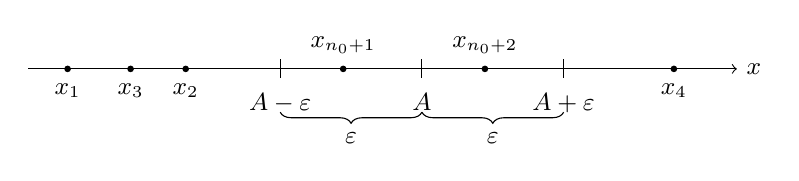
\begin{tikzpicture}[x=1cm, font=\small]
  \draw[->] (0,0) -- (9,0) node[right] {$x$};
  \foreach \x/\l in {0.5/x_1, 1.3/x_3, 2.0/x_2, 8.2/x_4}
    \fill (\x,0) circle (1.2pt) node[below=2pt] {$\l$};
  \foreach \x/\l in {3.2/A-\varepsilon, 5.0/A, 6.8/A+\varepsilon}
    \draw (\x,0.12) -- (\x,-0.12) node[below=2pt] {$\l$};
  \foreach \x/\l in {4.0/x_{n_0+1}, 5.8/x_{n_0+2}}
    \fill (\x,0) circle (1.2pt) node[above=2pt] {$\l$};
  \draw[decorate, decoration={brace, mirror, amplitude=4pt}] (3.2,-0.55) -- (5.0,-0.55) node[midway, below=4pt] {$\varepsilon$};
  \draw[decorate, decoration={brace, mirror, amplitude=4pt}] (5.0,-0.55) -- (6.8,-0.55) node[midway, below=4pt] {$\varepsilon$};
\end{tikzpicture}
\qquad
\begin{tikzpicture}[x=0.55cm, y=0.55cm, font=\small]
  \draw[->] (0,0) -- (8,0) node[right] {$n$};
  \draw[->] (0,0) -- (0,5.5) node[above] {$x$};
  \foreach \y/\l in {2.4/A-\varepsilon, 3.2/A, 4.0/A+\varepsilon}
    \draw[dashed] (0,\y) node[left] {$\l$} -- (7.5,\y);
  \fill (1,1.2) circle (1.2pt) node[below] {$x_1$};
  \fill (2,4.9) circle (1.2pt) node[above] {$x_2$};
  \fill (3,0.9) circle (1.2pt) node[below] {$x_3$};
  \fill (5,3.6) circle (1.2pt) node[above right] {$x_{n_0+1}$};
  \fill (6,2.9) circle (1.2pt) node[below right] {$x_{n_0+2}$};
\end{tikzpicture}
\end{center}

\textbf{Пример.} Доказать по определению, что
\[
  \lim_{n \to +\infty} \underbrace{\frac{2n + 5}{n + 1}}_{x_n} = \underbrace{2}_{A}.
\]
Возьмём произвольное $\varepsilon > 0$ и решим неравенство
$|x_n - A| < \varepsilon$:
\[
  |x_n - A| = \left| \frac{2n + 5}{n + 1} - 2 \right|
            = \left| \frac{2n + 5 - 2n - 2}{n + 1} \right|
            = \left| \frac{3}{n + 1} \right| = \frac{3}{n + 1} < \varepsilon;
\]
\[
  \frac{n + 1}{3} > \frac{1}{\varepsilon}, \qquad
  n + 1 > \frac{3}{\varepsilon}, \qquad
  n > \frac{3}{\varepsilon} - 1.
\]
Возьмём $n_0(\varepsilon) = \max\left\{1,\ \left[\tfrac{3}{\varepsilon} - 1\right]\right\}$,
тогда при $n > n_0$:
\[
  |x_n - A| = \frac{3}{n + 1} < \varepsilon.
\]
Таким образом, получили:
\begin{gather*}
  \forall \varepsilon > 0\ \exists n_0(\varepsilon) = \max\left\{1,\ \left[\tfrac{3}{\varepsilon} - 1\right]\right\}\
  \forall n \in \mathbb{N}\ \big(n > n_0 \to |x_n - A| < \varepsilon\big)\\
  \Longrightarrow\ \text{по определению предела } \lim_{n \to +\infty} x_n = A.
\end{gather*}
\begin{center}
\begin{tabular}{c|c|c|c|c}
  $\varepsilon$ & 1 & $\frac{1}{10}$ & $\frac{1}{100}$ & \dots \\ \hline
  $n_0$         & 2 & 29             & 299             & \dots \\
\end{tabular}
\end{center}

Если последовательность имеет конечный предел, то она называется
\underline{сходящейся}. В остальных случаях --- \underline{расходящейся}.

\subsection{Некоторые свойства сходящихся последовательностей}

\textbf{1$^\circ$.} Сходящаяся последовательность ограничена.

\dokstart Пусть задана сходящаяся последовательность $x_n$, т.\,е.
$\exists \lim\limits_{n \to +\infty} x_n = A$; тогда по определению предела
для $\varepsilon = 1$
\[
  \exists n_0(1)\ \forall n \in \mathbb{N}\ \big(n > n_0 \to A - 1 < x_n < A + 1\big).
\]
В качестве верхней границы для последовательности выберем
\[
  M = \max(A + 1,\ x_1,\ x_2,\ \dots,\ x_{n_0}),
\]
тогда $\forall n \in \mathbb{N}\ (x_n \le M)$. В качестве нижней границы
выберем
\[
  m = \min(A - 1,\ x_1,\ x_2,\ \dots,\ x_{n_0}),
\]
тогда $\forall n \in \mathbb{N}\ (x_n \ge m)$.\dokend

\textbf{2$^\circ$.} Если $\lim\limits_{n \to +\infty} x_n = A$, то
\[
  \forall P < A\ (\forall R > A)\ \exists n_0\ \forall n \in \mathbb{N}\
  \big(n > n_0 \to x_n > P\ (x_n < R)\big).
\]

\dokstart Докажем свойство для $P < A$. Выберем $\forall P < A$; т.\,к.
$\lim\limits_{n \to +\infty} x_n = A$, то по определению предела для
$\varepsilon = A - P$
\[
  \exists n_0\ \forall n \in \mathbb{N}\ \big(n > n_0 \to A - \varepsilon < x_n < A + \varepsilon\big).
\]
Т.\,к. $\varepsilon = A - P$, то $x_n > A - \varepsilon \to x_n > A - (A - P)
\to x_n > P$. Таким образом, получили:
\[
  \forall P < A\ \exists n_0\ \forall n \in \mathbb{N}\ \big(n > n_0 \to x_n > P\big).\ \blacktriangle
\]
% В тетради в итоговой строке написано ∀P>A — описка, по условию и доказательству должно быть ∀P<A.

\textbf{Замечание.} Из данного свойства следует, что если предел
последовательности положительный (отрицательный), то начиная с некоторого
номера все члены последовательности будут положительны (отрицательны).

\textbf{3$^\circ$.} Сходящаяся последовательность имеет единственный предел.

\dokstart Предположим противное: $\lim\limits_{n \to +\infty} x_n = A$ и
$\lim\limits_{n \to +\infty} x_n = B$, где $A < B$. Тогда возьмём число
$R = \dfrac{A + B}{2}$. Очевидно, что $R > A$ и $R < B$.

Т.\,к. $\lim\limits_{n \to +\infty} x_n = A$ и $R > A$, то по свойству
2$^\circ$
\[
  \exists n_1\ \forall n \in \mathbb{N}\ \big(n > n_1 \to x_n < R\big);
\]
т.\,к. $\lim\limits_{n \to +\infty} x_n = B$ и $R < B$, то
\[
  \exists n_2\ \forall n \in \mathbb{N}\ \big(n > n_2 \to x_n > R\big).
\]
Возьмём $n_0 = \max(n_1, n_2)$, тогда
\[
  \forall n \in \mathbb{N}\ \left(n > n_0 \to
  \begin{cases} x_n > R,\\ x_n < R \end{cases}\right)
  \ \Longrightarrow\ \text{противоречие}.
\]
Наше предположение было неверно; $A = B$, т.\,е. сходящаяся
последовательность имеет единственный предел.\dokend

\textbf{4$^\circ$.} Пусть $\lim\limits_{n \to +\infty} x_n = A$,
$\lim\limits_{n \to +\infty} y_n = B$ и $\forall n \in \mathbb{N}\ (x_n \le y_n)$.
Тогда $A \le B$.

\dokstart Предположим противное: $A > B$. Тогда $R = \dfrac{A + B}{2}$,
$B < R < A$.

Т.\,к. $R < A$ и $\lim\limits_{n \to +\infty} x_n = A$, то по 2$^\circ$
\[
  \exists n_1\ \forall n \in \mathbb{N}\ \big(n > n_1 \to x_n > R\big).
\]
Т.\,к. $R > B$ и $\lim\limits_{n \to +\infty} y_n = B$, то по 2$^\circ$
\[
  \exists n_2\ \forall n \in \mathbb{N}\ \big(n > n_2 \to y_n < R\big).
\]
$n_0 = \max(n_1, n_2)$:
\[
  \forall n \in \mathbb{N}\ \left(n > n_0 \to
  \begin{cases} x_n > R,\\ y_n < R \end{cases}\right),
\]
и, следовательно, при $n > n_0$: $y_n < x_n$, что противоречит условию
$x_n \le y_n$. Следовательно, наше предположение неверно и $A \le B$.\dokend

Данное свойство называется \underline{переходом к пределу в неравенствах}.

\textbf{5$^\circ$.} Пусть $\lim\limits_{n \to +\infty} x_n = A$,
$\lim\limits_{n \to +\infty} y_n = A$ и
$\forall n \in \mathbb{N}\ (x_n \le z_n \le y_n)$. Тогда
$\lim\limits_{n \to +\infty} z_n = A$.

\dokstart Выберем $\forall \varepsilon > 0$. Т.\,к.
$\lim\limits_{n \to +\infty} x_n = A$, то
\[
  \exists n_1\ \forall n \in \mathbb{N}\ \big(n > n_1 \to A - \varepsilon < x_n < A + \varepsilon\big).
\]
Т.\,к. $\lim\limits_{n \to +\infty} y_n = A$, то
\[
  \exists n_2\ \forall n \in \mathbb{N}\ \big(n > n_2 \to A - \varepsilon < y_n < A + \varepsilon\big).
\]
Возьмём $n_0 = \max(n_1, n_2)$. Тогда
\[
  \forall n \in \mathbb{N}\ \left(n > n_0 \to
  \begin{cases} A - \varepsilon < x_n,\\ x_n \le z_n \le y_n,\\ y_n < A + \varepsilon \end{cases}\right),
\]
\[
  A - \varepsilon < x_n \le z_n \le y_n < A + \varepsilon, \qquad
  A - \varepsilon < z_n < A + \varepsilon.
\]
Итак,
\[
  \forall \varepsilon > 0\ \exists n_0\ \forall n \in \mathbb{N}\
  \big(n > n_0 \to A - \varepsilon < z_n < A + \varepsilon\big),
\]
и, следовательно, по определению предела
$\lim\limits_{n \to +\infty} z_n = A$.\dokend

Это \underline{теорема о двух полицейских}.

\textbf{Замечание.} В свойствах 4$^\circ$ и 5$^\circ$ выполнение неравенств
$x_n \le y_n$ ($x_n \le z_n \le y_n$) достаточно потребовать начиная
с некоторого фиксированного номера $n$ (не обязательно с первого).


\subsection{Принцип вложенных и стягивающихся отрезков}
% лекция от 30.09.26 (дата в тетради); текст этого и следующих пунктов --- по тетради

\begin{definition}
  Последовательность отрезков $([a_n; b_n])$ называется
  \textbf{последовательностью стягивающихся отрезков}, если
  \[
    \lim_{n \to \infty} (b_n - a_n) = 0,
  \]
  то есть последовательность длин отрезков бесконечно малая.
\end{definition}

\begin{theorem}[принцип вложенных и стягивающихся отрезков]
  Любая последовательность вложенных и стягивающихся отрезков имеет
  единственную общую точку.
\end{theorem}

\begin{proof}
  Пусть задана последовательность вложенных и стягивающихся отрезков
  $([a_n; b_n])$.

  \begin{enumerate}
    \item Покажем, что общая точка существует.

    Обозначим через $A = \{a_n\}$ левые концы отрезков, а через
    $B = \{b_n\}$ --- правые концы.

    Так как $([a_n; b_n])$ --- последовательность вложенных отрезков, то
    $A \le B$ (все левые границы находятся левее правых границ).

    Тогда по аксиоме \textbf{непрерывности}
    \[
      \exists c\ (A \le c \le B).
    \]
    При этом $\forall n\ (a_n \le c \le b_n)$, то есть $c$ --- общая точка
    для всех отрезков.

    \item Докажем единственность общей точки.

    Предположим противное, что есть две общие точки $c$ и $d$, причём
    $c \ne d$. Тогда
    \[
      \forall n\ \left(
      \begin{cases}
        a_n \le c \le b_n,\\
        a_n \le d \le b_n
      \end{cases}
      \to\ 0 \le |c - d| \le b_n - a_n\right).
    \]
    Перейдём в неравенстве
    \[
      0 \le |c - d| \le b_n - a_n
    \]
    к пределу при $n \to \infty$.

    Так как $([a_n; b_n])$ --- последовательность стягивающихся отрезков, то
    \[
      \lim_{n \to +\infty} (b_n - a_n) = 0.
    \]
    Поэтому $0 \le |c - d| \le 0$. Следовательно,
    \[
      c = d.
    \]
    Наше предположение было неверно, и последовательность вложенных
    и стягивающихся отрезков имеет единственную общую точку.
  \end{enumerate}
\end{proof}


\subsection{Предельная точка. Подпоследовательности}

\begin{definition}
  Пусть заданы точка $x_0$ и число $\delta > 0$.
  \textbf{$\delta$-окрестностью} точки $x_0$ называется интервал
  \[
    U(x_0, \delta) = \{x \in \mathbb{R} : |x - x_0| < \delta\}
                   = (x_0 - \delta;\ x_0 + \delta).
  \]
\end{definition}

\begin{definition}
  Пусть задано непустое числовое множество $E$. Точка $x_0$ называется
  \textbf{предельной точкой} множества $E$, если в любой её окрестности есть
  бесконечно много точек из множества $E$.
\end{definition}

\begin{theorem}
  Любое бесконечное ограниченное множество имеет хотя бы одну предельную
  точку.
\end{theorem}

\begin{definition}
  Пусть заданы некоторая последовательность $(a_n)$ и возрастающая
  последовательность $(n_k)$. Тогда последовательность $(a_{n_k})$
  называется \textbf{подпоследовательностью} последовательности $(a_n)$.
\end{definition}

Например,
\[
  (a_n) = (n^2):\ 1,\ 4,\ 9,\ 16,\ \dots; \qquad
  (n_k) = (2k):\ 2,\ 4,\ 6,\ \dots; \qquad
  (a_{n_k}) = \big((2k)^2\big):\ 4,\ 16,\ 36,\ \dots
\]

\begin{theorem}[Больцано--Вейерштрасса]
  Из всякой ограниченной последовательности можно выделить сходящуюся
  подпоследовательность.
\end{theorem}

\begin{theorem}
  Если последовательность сходится к некоторому числу, то любая её
  подпоследовательность сходится к этому же числу.
\end{theorem}

\begin{remark}
  Из теоремы следует, что если из последовательности можно выделить две
  подпоследовательности, имеющие разные пределы, то она расходится, то есть
  не имеет конечного предела.
\end{remark}

\textbf{Пример.} $x_n = (-1)^n$.


\subsection{Предел монотонной последовательности}

Пусть $E$ --- непустое числовое ограниченное множество.

\begin{definition}
  Число $M_0$ называется \textbf{верхней гранью} (наименьшей верхней
  границей) множества $E$, если
  \begin{enumerate}
    \item $\forall x \in E\ (x \le M_0)$, то есть $M_0$ --- верхняя граница;
    \item $\forall \varepsilon > 0\ \exists x_1 \in E\ (x_1 > M_0 - \varepsilon)$,
      то есть $M_0$ --- наименьшая верхняя граница.
  \end{enumerate}
  \[
    M_0 = \sup E
  \]
\end{definition}

\begin{definition}
  Число $m_0$ называется \textbf{нижней гранью} (наибольшей нижней границей)
  множества $E$, если
  \begin{enumerate}
    \item $\forall x \in E\ (x \ge m_0)$, то есть $m_0$ --- нижняя граница;
    \item $\forall \varepsilon > 0\ \exists x_2 \in E\ (x_2 < m_0 + \varepsilon)$,
      то есть $m_0$ --- наибольшая нижняя граница.
  \end{enumerate}
  \[
    m_0 = \inf E
  \]
\end{definition}

\begin{theorem}
  Любое ограниченное множество имеет одну верхнюю и одну нижнюю грань.
\end{theorem}

\begin{theorem}[о пределе монотонной последовательности]
  Любая монотонная последовательность имеет предел (конечный или
  бесконечный).

  Причём если последовательность является неубывающей (невозрастающей)
  и ограничена сверху (снизу), то этот предел конечный. Если
  последовательность является неубывающей (невозрастающей) и не ограничена
  сверху (снизу), то этот предел равен $+\infty$ ($-\infty$).
\end{theorem}

\begin{proof}
  Для случая неубывающей последовательности, то есть
  $\forall n \in \mathbb{N}\ (a_n \le a_{n+1})$.

  \begin{enumerate}
    \item Последовательность $(a_n)$ ограничена.

    Тогда множество её значений имеет верхнюю грань. Пусть
    $A = \sup (a_n)$.

    Выберем $\forall \varepsilon > 0$. По определению верхней грани
    \[
      \forall n\ (a_n \le A < A + \varepsilon).
    \]
    По определению верхней грани
    \[
      \exists n_0\ (a_{n_0} > A - \varepsilon).
    \]
    Так как последовательность неубывающая, то
    $\forall n\ (n > n_0 \to a_n \ge a_{n_0})$. Следовательно,
    $a_n \ge a_{n_0} > A - \varepsilon$, тогда
    % В тетради здесь a_{n_0} \ge A - \varepsilon --- описка: строкой выше a_{n_0} > A - \varepsilon.
    \[
      \forall n\ \big(n > n_0 \to A - \varepsilon < a_n < A + \varepsilon\big)
      \quad\text{или}\quad |a_n - A| < \varepsilon.
    \]
    Получили
    \[
      \forall \varepsilon > 0\ \exists n_0\ \forall n\
      \big(n > n_0 \to |a_n - A| < \varepsilon\big).
    \]
    Следовательно, $\lim\limits_{n \to \infty} a_n = A$.

    \item Последовательность $(a_n)$ не ограничена сверху.

    Тогда по определению неограниченной последовательности
    \[
      \forall \varepsilon > 0\ \exists n_0 \in \mathbb{N}\ (a_{n_0} > \varepsilon).
    \]
    Так как последовательность неубывающая, то
    \[
      \forall n\ (n > n_0 \to a_n \ge a_{n_0} > \varepsilon).
    \]
    Тогда по определению бесконечно большой последовательности
    $\lim\limits_{n \to \infty} a_n = +\infty$.
  \end{enumerate}
\end{proof}


\subsection{Второй замечательный предел}

\begin{theorem}
  Последовательность $(a_n)$, где $a_n = \left(1 + \dfrac{1}{n}\right)^n$,
  имеет конечный предел.
\end{theorem}

\begin{proof}
  Используем формулу бинома Ньютона:
  \begin{multline*}
    (a + b)^n = a^n + n\cdot a^{n-1}b + \frac{n(n-1)}{2!}\,a^{n-2}b^2
      + \frac{n(n-1)(n-2)}{3!}\,a^{n-3}b^3 + {} \\
      + \frac{n(n-1)(n-2)(n-3)}{4!}\,a^{n-4}b^4 + \dots
      + \frac{n(n-1)(n-2)\cdot\ldots\cdot(n-n+1)}{n!}\,b^n.
  \end{multline*}
  $a_n = \left(1 + \dfrac{1}{n}\right)^n$, поэтому $a = 1$ и
  $b = \dfrac{1}{n}$. Используем формулу бинома Ньютона:
  \begin{align*}
    a_n = \left(1 + \frac{1}{n}\right)^n
      &= 1 + n\cdot\frac{1}{n} + \frac{n(n-1)}{2!}\cdot\frac{1}{n^2} + \dots
        + \frac{n(n-1)(n-2)\cdot\ldots\cdot(n-n+1)}{n!}\cdot\frac{1}{n^n} = \\
      &= 2 + \frac{1}{2!}\left(1 - \frac{1}{n}\right)
        + \frac{1}{3!}\left(1 - \frac{1}{n}\right)\left(1 - \frac{2}{n}\right)
        + \frac{1}{4!}\left(1 - \frac{1}{n}\right)\left(1 - \frac{2}{n}\right)\left(1 - \frac{3}{n}\right)
        + \dots + {} \\
      &\quad + \frac{1}{n!}\left(1 - \frac{1}{n}\right)\left(1 - \frac{2}{n}\right)
        \cdot\ldots\cdot\left(1 - \frac{n-1}{n}\right).
  \end{align*}
  \textbf{(!)} Заменим каждую скобку большим числом --- единицей:
  % В тетради второй знак тоже <; строго верно \le (при n = 2 там равенство).
  \begin{align*}
    a_n &< 2 + \frac{1}{2!} + \frac{1}{3!} + \frac{1}{4!} + \dots + \frac{1}{n!}
         \le 2 + \frac{1}{2} + \frac{1}{4} + \frac{1}{2^3} + \dots + \frac{1}{2^{n-1}} = \\
        &= 2 + \frac{\frac12\left(1 - \left(\frac12\right)^{n-1}\right)}{1 - \frac12}
         = 3 - \left(\frac12\right)^{n-1} < 3
  \end{align*}
  (сумма геометрической прогрессии: $S_n = \dfrac{b_1(1 - q^n)}{1 - q}$).

  Таким образом, $\forall n\ (a_n < 3)$, то есть последовательность $(a_n)$
  ограничена сверху.
  % На этом запись в тетради заканчивается --- продолжение доказательства будет дописано по следующей лекции.
\end{proof}

\end{document}
